\documentclass[11pt]{article}
\usepackage[margin=1in]{geometry}
\usepackage{amsmath,amssymb,amsfonts}
\usepackage{graphicx,float}
\usepackage{fancyhdr,booktabs}
\usepackage{listings}
\usepackage{hyperref}
\usepackage{listings, soul}
\usepackage[most]{tcolorbox}
\tcbset{breakable}
\usepackage{tikz}
\usetikzlibrary{arrows.meta, positioning, calc}

\lstset{
    language=Matlab,
    basicstyle=\ttfamily\small,
    breaklines=true,
    keepspaces=true,
    showstringspaces=false
}



\begin{document}
\subsection*{Problem 8.} Add compensation to improve the closed loop behavior (both transient and steady-state response).  Describe your process, the compensation selected and how you improved the response compared to the uncompensated system.\\\\
\underline{Understand the uncompensated system}
\begin{center}
    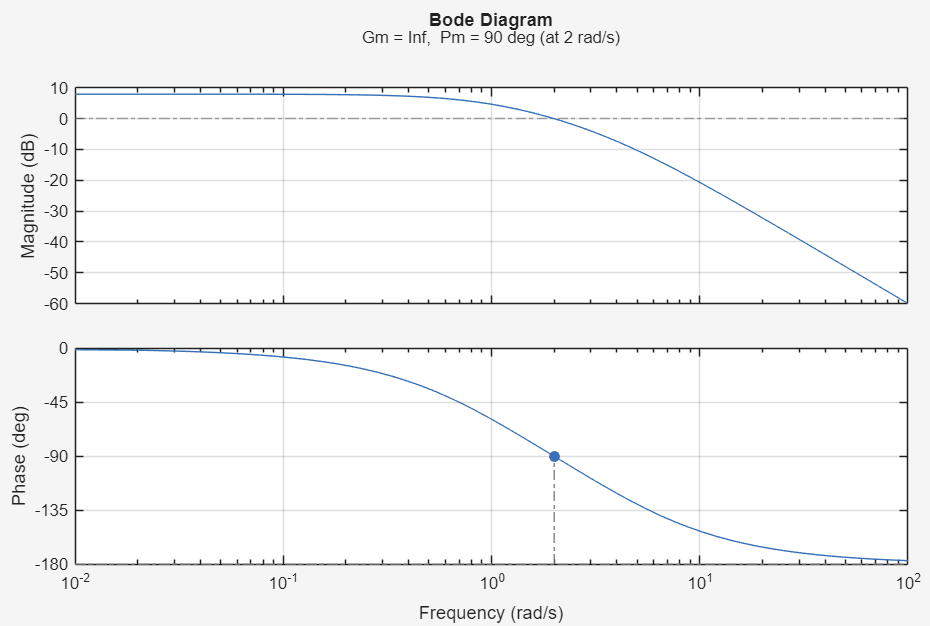
\includegraphics[width=0.7\textwidth]{../P8-1.png}
\end{center}
The uncompensated system has a gain crossover frequency of $\omega_{gc}=2$ rad/s and a phase margin of 90 degrees.\\\\
\textit{I can add a lead compensator to maintain a decent phase margin while improving system response speed by increasing gain $K_c$. I will arbitrarily decide on a phase margin of 45 degrees.}
\begin{center}
    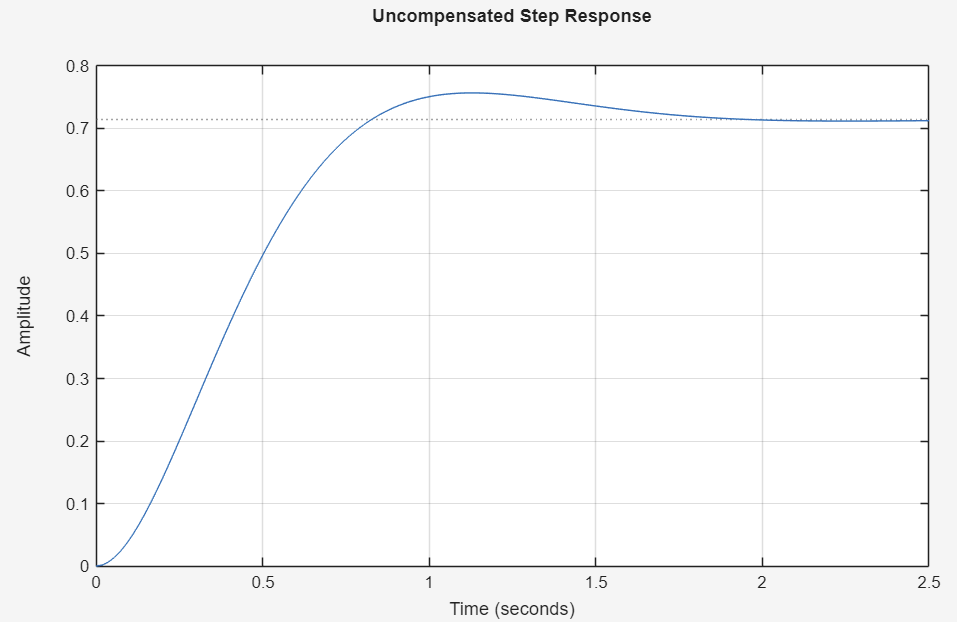
\includegraphics[width=0.7\textwidth]{../P8-2.png}
\end{center}
\newpage
From MATLAB, the step-response time specs are as follows:
\begin{lstlisting}
         RiseTime: 0.5435
    TransientTime: 1.6066
     SettlingTime: 1.6066
      SettlingMin: 0.6454
      SettlingMax: 0.7568
        Overshoot: 5.9523
       Undershoot: 0
             Peak: 0.7568
         PeakTime: 1.1237

Steady-state error: 0.2857
\end{lstlisting}
Since there is a steady-state error, I can add a lag compensator to reduce the steady-state error to a unit step input.
\begin{itemize}
    \item[1] \textbf{Determine lead compensator parameters:} I will choose an arbitrary lead compensator zero and pole location of $z=2$ and $p=8$, such that $z<p$.\\\\
    In MATLAB, I will iteratively increase the gain $K_c$ until the phase margin is 45 degrees, aiming for a higher crossover frequency of about double the uncompensated system's crossover frequency ($\omega_{gc,\text{ desired}} \approx 4$ rad/s).
    \begin{center}
        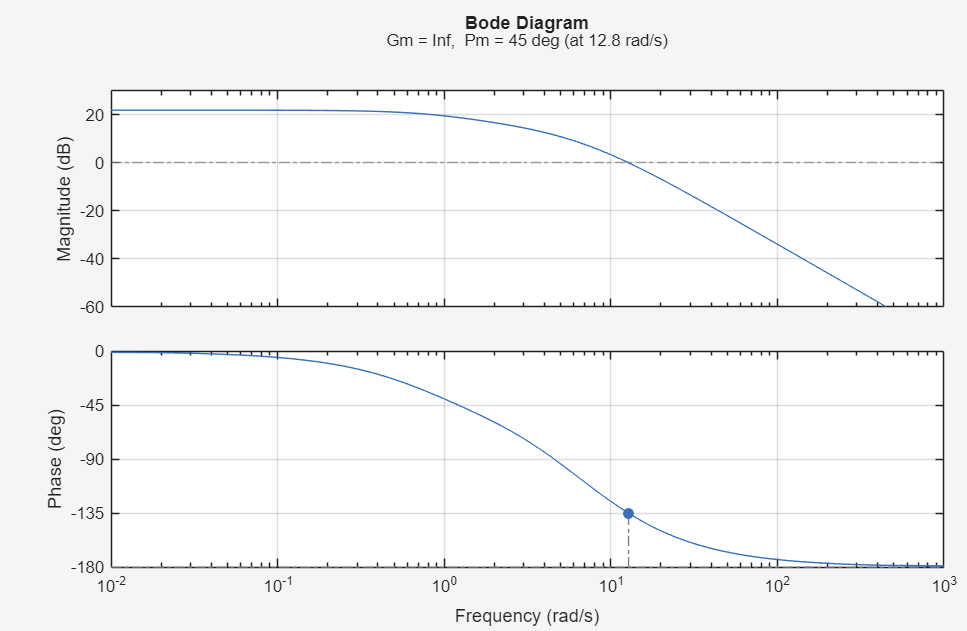
\includegraphics[width=0.7\textwidth]{../P8-3.png}
    \end{center}
    For $K_c=20$, I found that
    \begin{lstlisting}
        Gain crossover: 12.78 rad/s
        Phase margin: 45.02 degrees
    \end{lstlisting}
    This is satisfactory, so I will keep the lead compensator parameters as $K_c=20$, $z=2$, and $p=8$.
    \item[2] \textbf{Determine lag compensator parameters:} Solving the steady-state error of the lead compensated system:
    \[
L(s)=\frac{20(s+2)}{s+8}\cdot\frac{10}{(s+1)(s+4)}=\frac{200(s+2)}{(s+8)(s+1)(s+4)}
\]
For a unit step input, the steady-state error is:
\[
\begin{aligned}
e_{ss}
&= \lim_{s\to 0}sE(s)\\
&= \lim_{s\to 0}s\cdot\frac{1}{s}\cdot\frac{1}{1+L(s)}\\
&= \lim_{s\to 0}
\frac{(s+8)(s+1)(s+4)}
{(s+8)(s+1)(s+4)+200(s+2)}\\
&= \frac{32}{32+400}\\
&= \boxed{\frac{2}{27}\approx 0.0741}.
\end{aligned}
\]
Thus, I will need to add a lag compensator to limit the steady-state error to a unit step input to be less than or equal to 0.01. Finding the ratio $z/p$ for the lag compensator:
\[C_{lag} = \frac{s+z}{s+p}\]
\[
\begin{aligned}
e_{ss}
&= \lim_{s\to 0}sE(s)\\
&= \lim_{s\to 0}s\cdot\frac{1}{s}\cdot\frac{1}{1+L(s)}\\
&= \lim_{s\to 0}
\frac{(s+8)(s+1)(s+4)(s-p)}
{(s+8)(s+1)(s+4)(s-p)+200(s+2)(s-z)}\\
&= \frac{-32p}{-32p+400z}\\
&= \frac{32p}{32p+400z}
\end{aligned}
\]
\[
\begin{aligned}
e_{ss} &= \frac{32p}{32p+400z}\leq 0.01\\
32p &\leq 0.32p+4z\\
31.68p &\leq 4z\\
\frac{z}{p} &\geq 7.92
\end{aligned}
\]
\end{itemize}
To keep the lag compensator's poles and zeros close to the origin, pick $p=0.1$ and $z=0.792$.
\newpage
\textbf{Final Compensated Response}
\begin{center}
    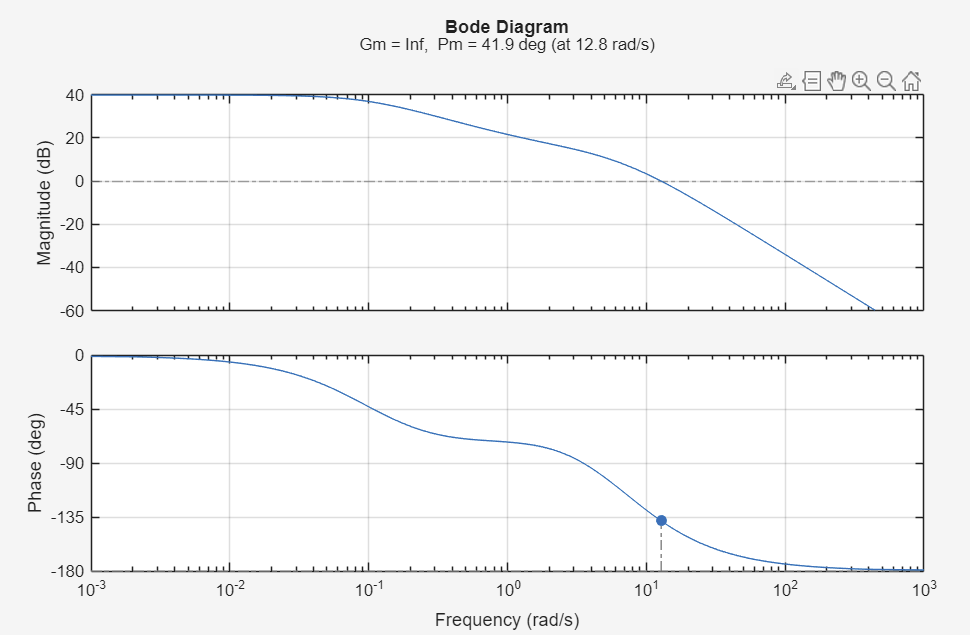
\includegraphics[width=0.9\textwidth]{../P8 final.png}
\end{center}
\begin{center}
    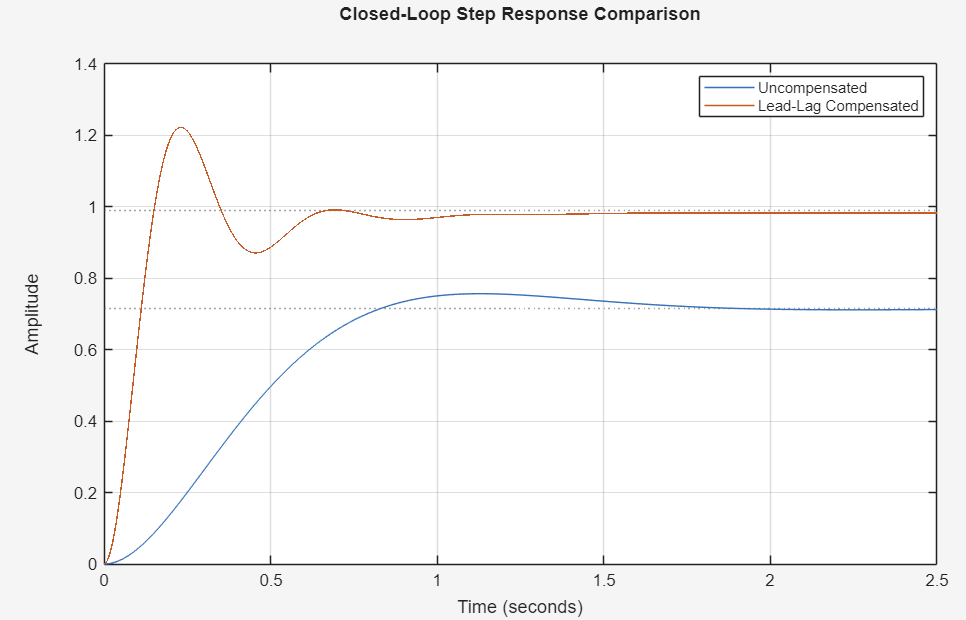
\includegraphics[width=0.9\textwidth]{../P8 final-1.png}
\end{center}
Time specs:
\begin{lstlisting}
    Lead-Lag Compensated specs:
Gain crossover: 12.7911 rad/s
Phase margin: 41.88 degrees

ans = 

  struct with fields:

         RiseTime: 0.1013
    TransientTime: 1.0000
     SettlingTime: 1.0000
      SettlingMin: 0.8712
      SettlingMax: 1.2229
        Overshoot: 23.5227
       Undershoot: 0
             Peak: 1.2229
         PeakTime: 0.2299

Steady-state error: 0.0100
\end{lstlisting}
\end{document}
